\documentclass[border=1pt]{standalone}
\usepackage{tikz}
\usepackage[compat=1.0.0]{tikz-feynman}
\usepackage{contour}

\begin{document}
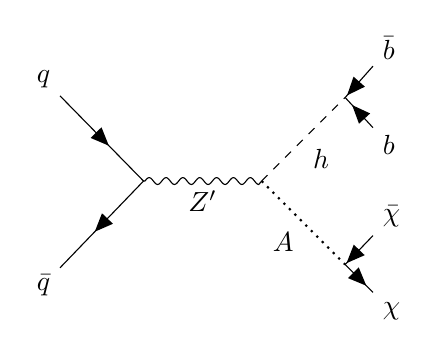
\begin{tikzpicture}[node distance=0.5cm]
      \begin{feynman}
          \vertex (a);
          \vertex [above left=of a](p1){\(q\)};
          \vertex [below left=of a](p2){\(\bar{q}\)};
          \vertex [right=of a] (b);
          \vertex [above right=of b] (d);
          \vertex [below right=of b] (c);
          \vertex [above right=.5cm of d] (f4) {\(\bar{b}\)};
          \vertex [below right=.5cm of d] (f5) {\(b\)};
          \vertex [above right=.5cm of c] (f2) {\(\bar{\chi}\)};
          \vertex [below right=.5cm of c] (f3) {\(\chi\)};
          \diagram*{
      (p1) -- [fermion] (a) -- [fermion] (p2),
                (a) -- [boson, edge label'=\(Z'\)] (b) ,
                (b) -- [scalar, edge label'=\(h\)]  (d),
                (f5) -- [fermion](d)--[anti fermion](f4),
          (b) -- [ghost, edge label'=\(A\)] (c),
          (c) -- [anti fermion] (f2),
          (c) -- [fermion] (f3),
      };
  \end{feynman}
\end{tikzpicture}
\end{document}
